\documentclass{article} 
    %\usepackage[margin=0.8in]{geometry}
    %\usepackage[parfill]{parskip}
    \usepackage[utf8]{inputenc}
    \usepackage{graphicx}
    \usepackage{siunitx}
    \usepackage{amsmath}
    \usepackage{listings}
    \usepackage{color}
    \usepackage{cleveref}


% Letternumbering
\renewcommand{\thesection}{\Roman{section}} 

\title{Artificial Intelligence Methods, exercise 4}
\author{Rendell Cale}
\date{\today}

\begin{document}

\maketitle

\section{}
\begin{centering}
	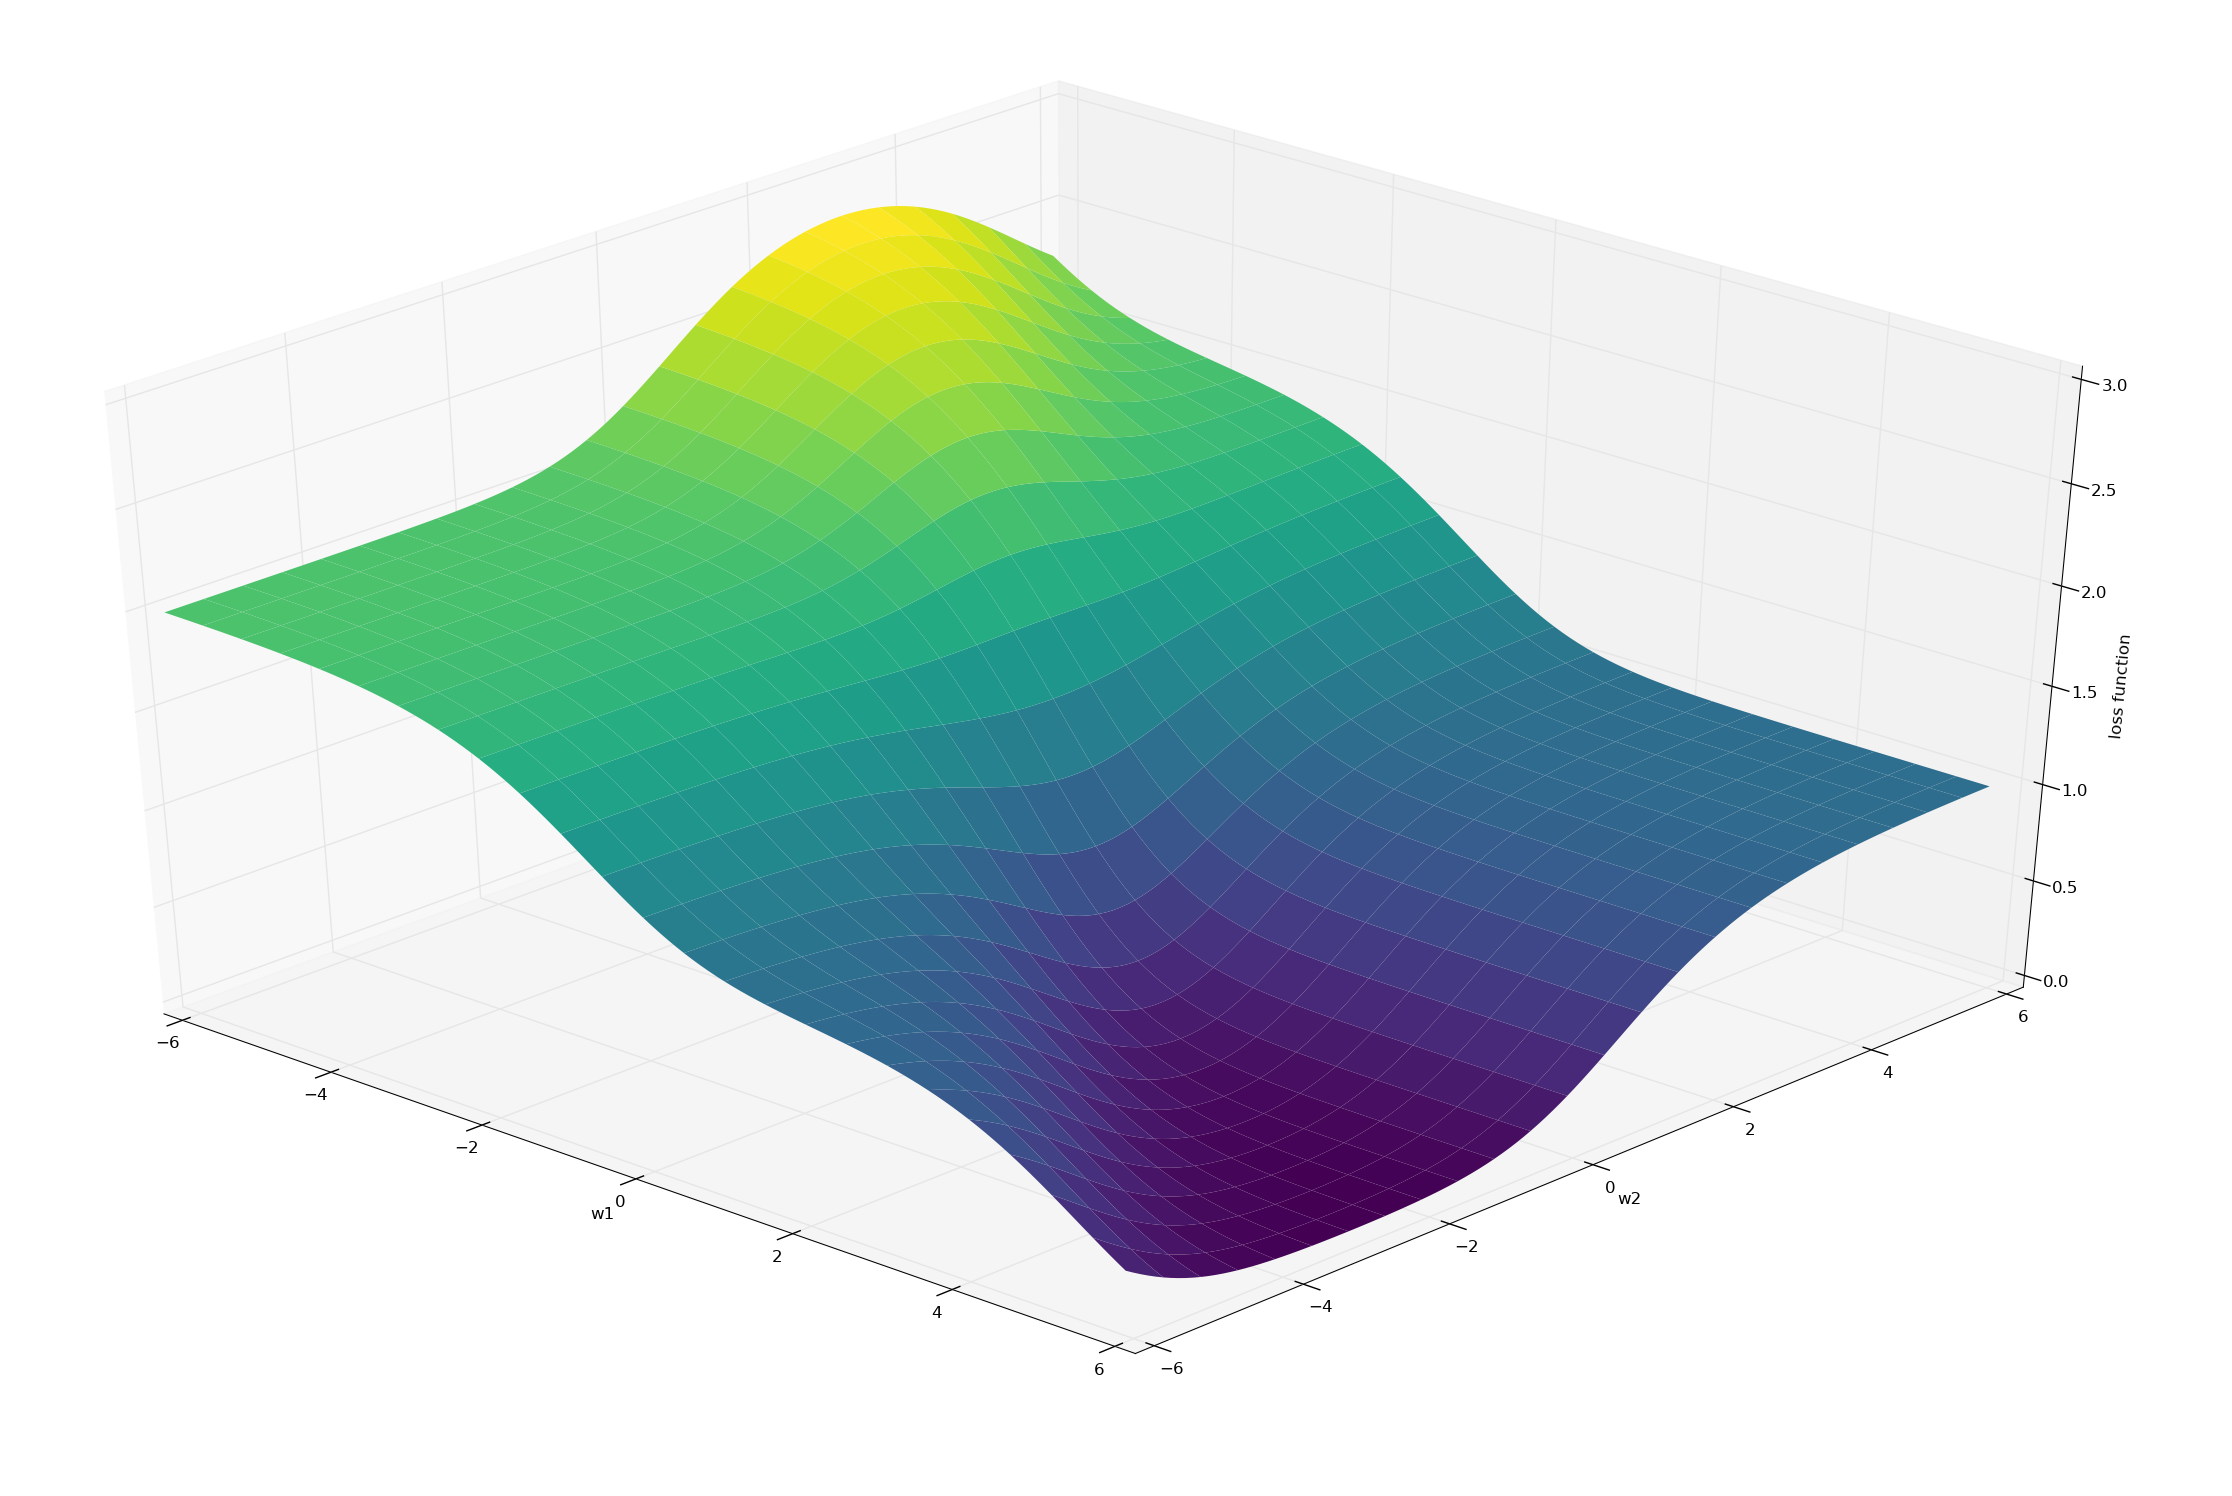
\includegraphics[width=\linewidth]{exercise4_task1.png}
\end{centering}

From the plot it does not seem that there is a definite lowest point, but rather that the function decreases monotonically toward zero in the as $w=(w_1,w_2)=(w, -w)$ and $w \rightarrow \infty$. 

\subsection{}

\subsection{}
Using the definitions for $\sigma(w,x)$ and $L_{simple}(w)$,
\begin{align}
	\sigma(w,x) &= \frac{1}{1 + e^{-w^Tx}} \\
	L_{simple} &= \left[ \sigma(w,[1,0]) - 1 \right]^2 + \sigma(w,[0,1])^2 + \left[ \sigma(w,[1,1]) - 1 \right]^2,
\end{align}
we can compute the gradient of $L_{simple}$, $\nabla_w L_{simple}$.

We begin by writing out the expression using $w = [w_1, w_2]^T$.

\begin{align}
	L_{simple} &= \left[ \frac{1}{1 + e^{-w_1}} - 1 \right]^2 + \left[ \frac{1}{1 + e^{-w_2}} \right]^2 + \left[ \frac{1}{1 + e^{-w_1 - w_2}} - 1 \right]^2 \\
	&= \left[ \sigma(w_1) - 1 \right]^2 + \sigma(w_2)^2 + \left[ \sigma(w_1 + w_2) - 1 \right]^2.
\end{align}

It is quite well known that
\begin{equation}
	\frac{\partial \sigma(x)}{\partial x} = \sigma(x) (1 - \sigma(x))
\end{equation}

Using this and the chain rule, we find that
\begin{align}
	\frac{\partial L_{simple}}{\partial w_1}(w) = 2 \left[ \sigma(w_1) - 1 \right]  \frac{\partial \sigma(w_1)}{\partial w_1}  + 2 \left[ \sigma(w_1 + w_2) - 1 \right] \frac{\partial \sigma(w_1 + w_2)}{\partial w_1} \\
	= 2 (\sigma(w_1) - 1)\sigma(w_1)(1 - \sigma(w_1)) + 2 (\sigma(w_1 + w_2) - 1) \sigma(w_1 + w_2)(1 - \sigma(w_1+w_2)) \\
	= -2 \left[ \sigma(w_1) - 1 \right]^2\sigma(w_1) -2 \left[ \sigma(w_1 + w_2) - 1 \right]^2\sigma(w_1 + w_2).
\end{align}

For $w_2$ we get
\begin{align}
	\frac{\partial L_{simple}}{\partial w_2}(w) &= 2\sigma(w_2)\sigma(w_2)(1 - \sigma(w_2)) + 2 \left[ \sigma(w_1 + w_2) - 1 \right] \sigma(w_1+w_2)(1 - \sigma(w_1 + w_2)) \\
	&= 2 \sigma(w_2)^2(1 - \sigma(w_2)) - 2 \sigma(w_1+w_2) \left[ \sigma(w_1+w_2) - 1 \right]^2.
\end{align}

\subsection{}
After implementing the update rule in Python, starting the weights at $(w_1,w_2) = (0,0)$, running it for $10000$ iterations and plotting the surface along with the search results for different $\eta$, I get:

\begin{centering}
	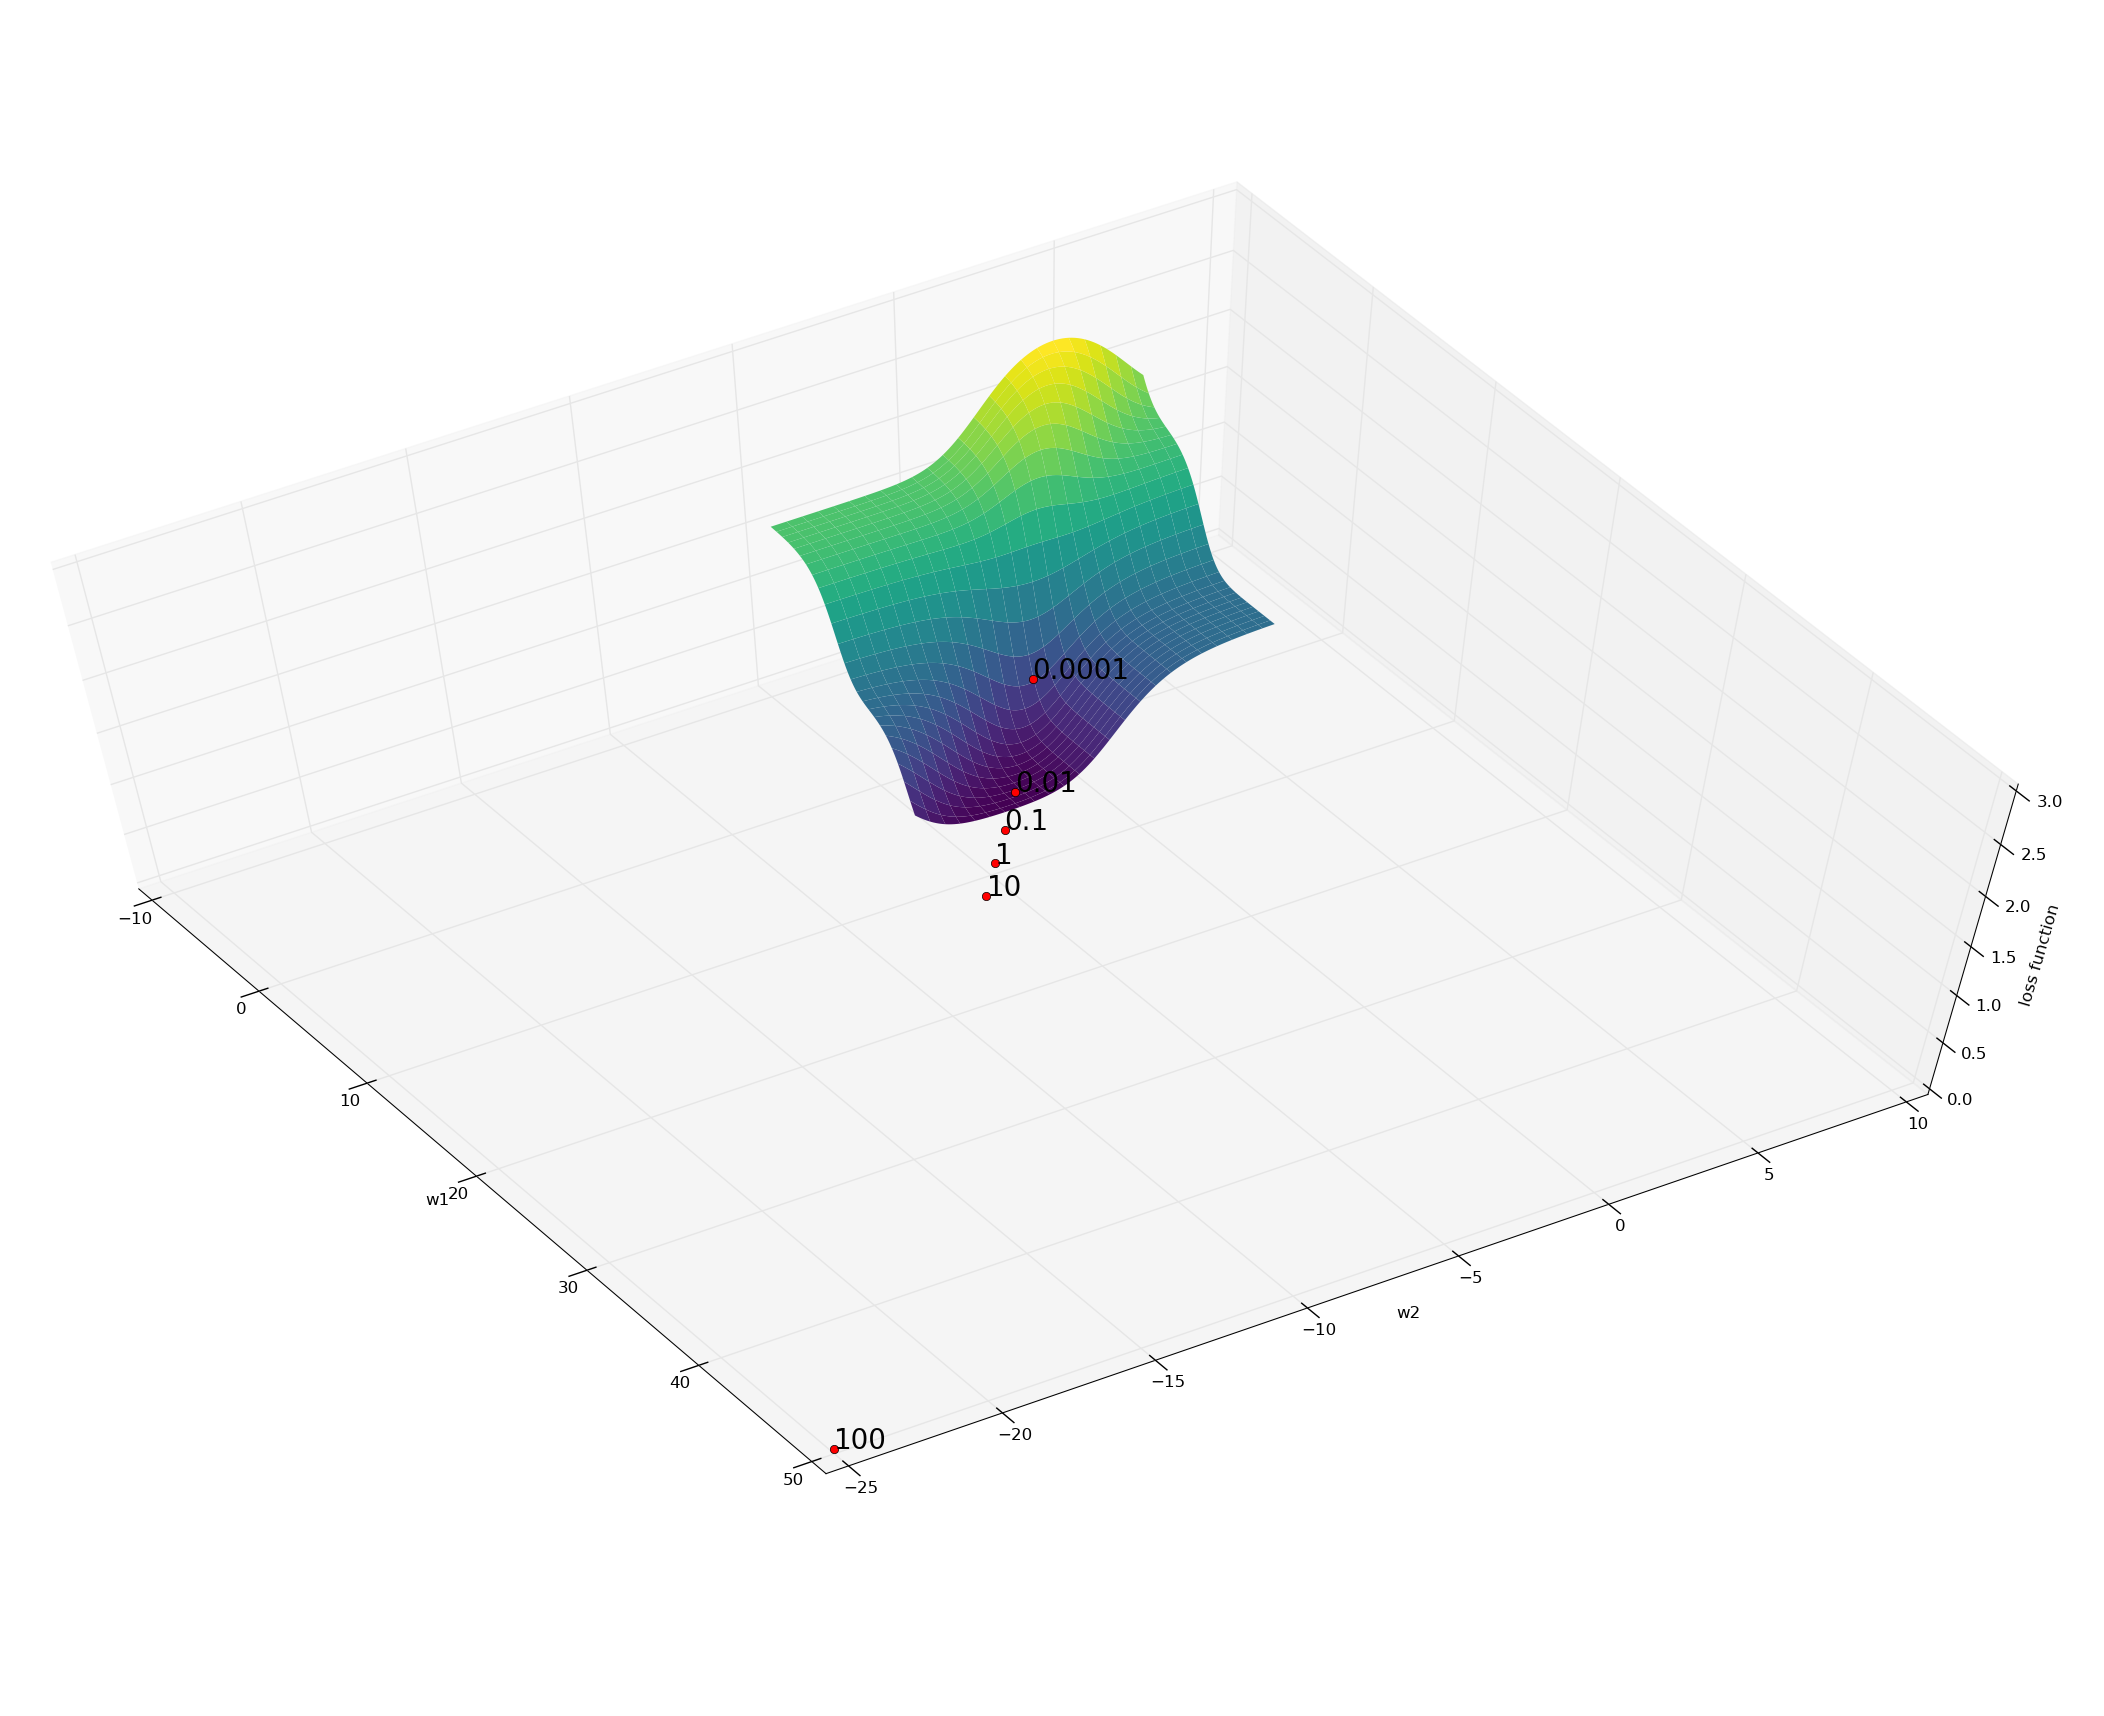
\includegraphics[width=\linewidth]{exercise4_task13.png}
\end{centering}

Notice in the plot that there is quite a big difference between the different choices of $\eta$. With $\eta = 100$ the weights ended up quite far away from the others, but actually the difference in the loss function values of the resulting points isn't that big when we compare $\eta = 100$ to $\eta = 0.01$. 
The function does decrease in the direction of $(w_1,w_2) \rightarrow (\infty,-\infty)$, but is essentially constantly zero from quite early on. 

Another interesting thing we can see from this plot is that for $\eta=0.0001$, the loss function is significantly larger. This is probably since the sequence converges slower for small values of $\eta$. 

\section{}
\subsection{Derivative formula}
Using the chain rule, we find
\begin{equation} 
	\frac{\partial L_n}{\partial w_i} = (\sigma(w,x_n) - y_n) \frac{\partial \sigma(w,x_n)}{\partial w_i} \label{eq:partial_L_halway}
\end{equation}

Computing the derivative of $\sigma(w,x_n)$ gives
\begin{align}
	\frac{\partial \sigma(w,x_n)}{\partial w_i} &= \frac{\partial}{\partial w_i}\left( \frac{1}{1+e^{-w^Tx_n}} \right) \\
	&= \frac{-1}{(1+e^{-w^T x_n})^2} \frac{\partial}{\partial w_i}(1 + e^{-w^Tx_n}) \\
	&= \sigma(w,x_n)^2 x_i e^{-w^T x_n}
\end{align}

Using this in \cref{eq:partial_L_halway} gives the final formula which we'll use for the remainder of the task. 
\begin{align}
	\frac{\partial L_n}{\partial w_i} &= (\sigma(w,x_n) - y_n) \frac{\partial \sigma(w,x_n)}{\partial w_i}  \\
	&= x_i (\sigma(w,x_n) - y_n) \sigma(w,x_n)^2 e^{-w^T x_n}
\end{align} 

\subsection{Experiments}
\subsubsection{General results}
After implementing the algorithms and experimenting a bit, it seems clear that both of them work but they behave differently when it comes to convergence and time requirements. The big advantage with Batch Gradient Descent (BGD) is that it takes into account all of the data when it computes the gradient. This makes for a more stable and correct algorithm but comes at the cost of time requirements, especially as the dataset gets large. 
Stochastic Gradient Descent (SGD) is able to obtain almost the same error rate as BGD, but it achieves it alot faster in time. For instance when training in the small seperable dataset with a learning rate of 1.0, BGD was able to achieve a zero errors in less than 50 iterations taking 6.5 seconds , whereas SGD required more than 100 iterations taking 0.07 seconds. 

The general trend is that the non-seperable datasets are harder to train on, since both BGD and SGD required more iterations to get low error scores there. It was also quite noticable with BGD that the size og the datasets directly affected the speed of the algorithm. There was also some effect of dataset size with SGD, but it wasn't nearly as significant, so I suspect it is more the result of implementation details rather than algorithmic time requirements. 

\subsubsection{Scatter plot}
I trained the perceptron on the big non-seperable dataset using Stochastic Gradient Descent. The following scatter plot shows the two classes of points and the line which attempts to divide them. 

\begin{centering}
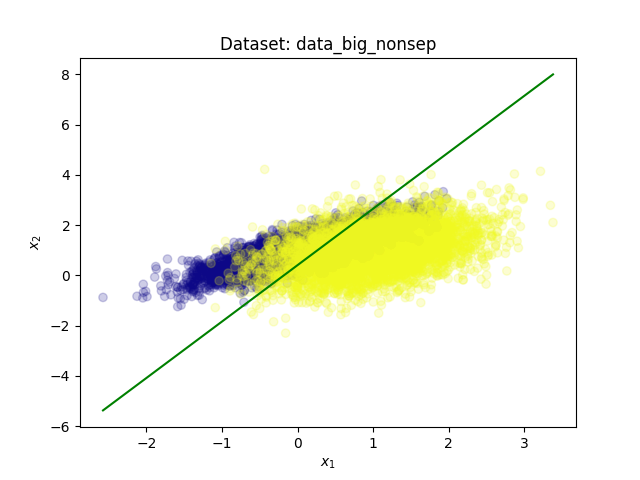
\includegraphics[width=0.9\linewidth]{ex4_scatter_training.png}
\end{centering}

Using the same line on the test data yields the following plot.

\begin{centering}
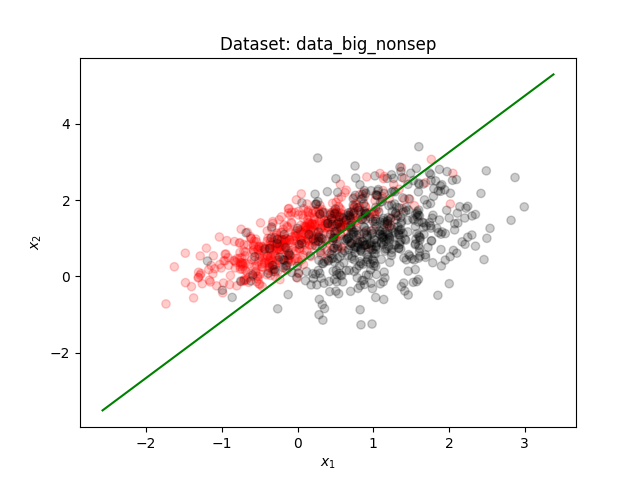
\includegraphics[width=0.9\linewidth]{ex4_scatter_test.png}
\end{centering}

Combining both plots give the following.

\begin{centering}
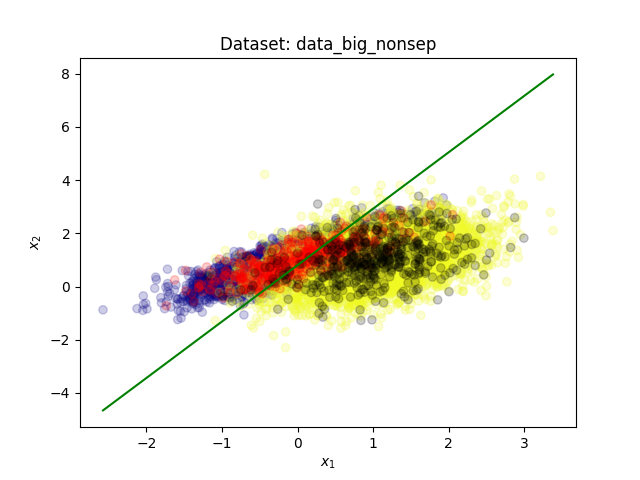
\includegraphics[width=0.9\linewidth]{ex4_scatter_both.png}
\end{centering}

\subsubsection{Effects of iterations}
The general effect that increasing the number of iterations is that the error goes down, but only to a certain point. For the seperable datasets it was quite easy to get the error down to 0, which makes sense, but for the non-seperable datasets the error will converge to something non-zero and bounce slightly up or down for each iteration. 

To see this we will plot the error as a function of the number of iterations for the small non-seperable dataset. 

\begin{centering}
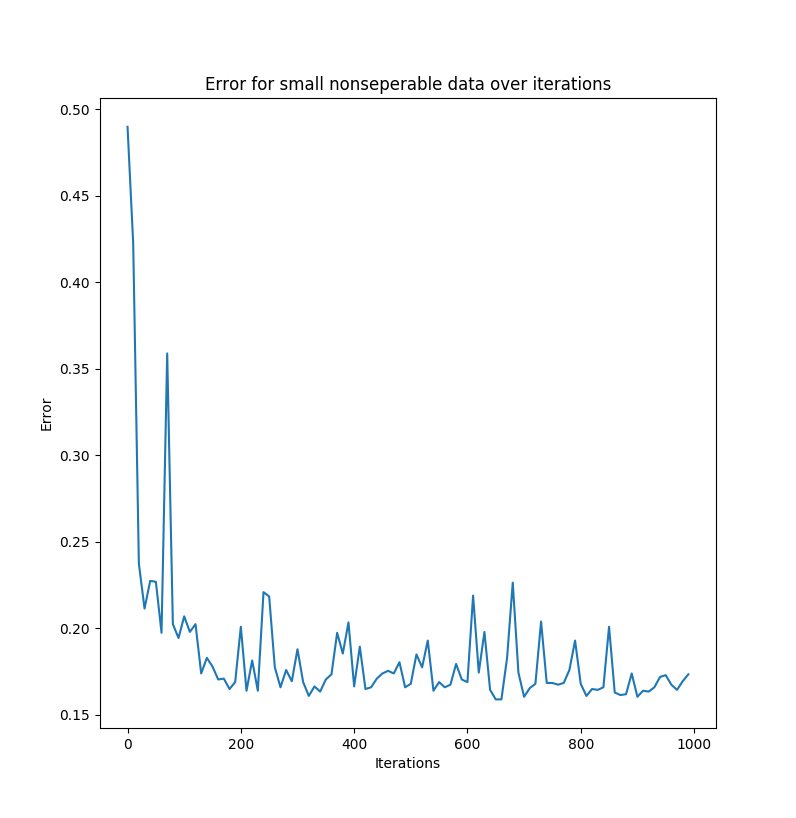
\includegraphics[width=0.9\linewidth]{ex4_error_over_iterations_sgc.png}
\end{centering}

As we can see the error rate converges around 16\% and jumps a bit up and down between each iteration. These results were obtained using the Stochastic training method so it is reasonable that the errors spike from time to time. 
I suspected that using Batch gradient descent would give more stable convergence. To test this a ran the same method on the same dataset for the same number of iterations. This gave a much more stable convergence.

\begin{centering}
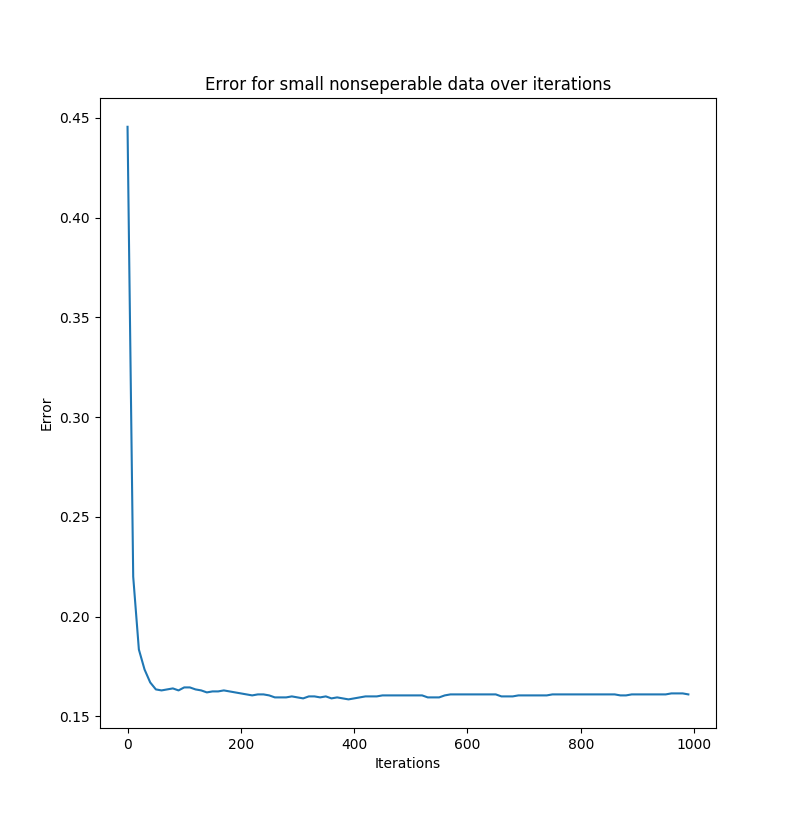
\includegraphics[width=0.9\linewidth]{ex4_error_over_iterations_bgc.png}
\end{centering}

Of course the cost of this stability is that the training time went from 0.37 seconds with SGD to 137 seconds with BGD.


\end{document}

